\documentclass{article}

\usepackage[english, russian]{babel}
\usepackage{geometry}
\usepackage{graphicx}
\usepackage{listings}
\usepackage{xcolor}
\usepackage[14pt]{extsizes}
\usepackage{amsmath}
\usepackage{setspace}
\usepackage{multirow}
\usepackage{tocloft}
\usepackage{indentfirst} 
\usepackage{lipsum}
\usepackage{caption}
\usepackage{cmap}
\usepackage[utf8]{inputenc}
\usepackage[T2A]{fontenc}
\usepackage{svg}

\captionsetup[figure]{name={Рисунок},labelsep=endash}
\captionsetup[table]{singlelinecheck=false, labelsep=endash}

\renewcommand{\cftsecleader}{\cftdotfill{\cftdotsep}}
\geometry{pdftex, left = 3cm, right = 1cm	, top = 2cm, bottom = 2cm}
\onehalfspacing

\setlength{\parindent}{1,25cm}
\lstdefinestyle{python}{
	language={Python},
	basicstyle=\footnotesize\ttfamily,
	frame=single,
	tabsize=4,	
	breaklines=true
}

\DeclareCaptionLabelSeparator{line}{\ --\ }
\DeclareCaptionFont{white}{\color{white}}
\DeclareCaptionFormat{listing}{\colorbox[cmyk]{0.43,0.35,0.35,0.01}{\parbox{\textwidth}{\hspace{15pt}#1#2#3}}}
\captionsetup[lstlisting]{
	singlelinecheck=false,
	labelsep=line
}

\begin{document}
\begin{titlepage}
	\newgeometry{pdftex, left=2cm, right=2cm, top=2.5cm, bottom=2.5cm}
	\fontsize{12pt}{12pt}\selectfont
	\noindent\begin{tabular}{|c|c|}	\hline
	\noindent\begin{minipage}{0.15\textwidth}
		
\includegraphics[width=\linewidth]{tools/logo.png}
	\end{minipage} &
	\noindent\begin{minipage}{0.85\textwidth}\centering
		\textbf{\newline Министерство науки и высшего образования Российской Федерации}\\
		\textbf{Федеральное государственное бюджетное образовательное учреждение высшего образования}\\
		\textbf{«Московский государственный технический университет имени Н.Э.~Баумана}\\
		\textbf{(национальный исследовательский университет)»}\\
		\textbf{(МГТУ им. Н.Э.~Баумана)}
	\end{minipage} \\
	\hline	\end{tabular}\newline\newline\newline
	\noindent ФАКУЛЬТЕТ \underline{«Информатика и системы управления»} \newline\newline
	\noindent КАФЕДРА \underline{«Программное обеспечение ЭВМ и информационные технологии»}\newline\newline\newline\newline\newline\newline

	\noindent\begin{minipage}{1.0\textwidth}\centering
		\Large\textbf{       Практикум №2}
		\end{minipage}
		
	\noindent\begin{minipage}{1.0\textwidth}\centering
		\textbf{\newline}	
		\end{minipage}

	\noindent\begin{minipage}{1.0\textwidth}\centering
		\Large\textbf{по дисциплине «Архитектура ЭВМ»}	
		\end{minipage}
		
	\noindent\begin{minipage}{1.0\textwidth}\centering
		\Large\textbf{\newline\newline\newline\newline}	
		\end{minipage}
	
	\noindent\textbf{Тема} \underline{Обработка и визуализация графов в вычислительном комплексе Тераграф}
\newline\newline
	\textbf{Студент} \underline{Тузов Даниил Александрович}\newline\newline
	\textbf{Группа} \underline{ИУ7-52Б}\newline\newline
	\textbf{Преподаватель} \underline{Калитвенцев Максим Павлович}
	
	\begin{center}
		\vfill
		Москва, \the\year ~г.
	\end{center}
	\restoregeometry
	\clearpage
\end{titlepage}

\section{Введение}

Практикум посвящен освоению принципов представления графов и их обработке с помощью вычислительного комплекса 
Тераграф. В ходе практикума необходимо ознакомиться с вариантами представления графов в виде объединения структур языка 
$C/C++$, изучить и применить на практике примеры решения некоторых задач на графах. По индивидуальному варианту 
необходимо разработать программу хост-подсистемы и программного ядра $sw_kernel$, выполняющего обработку и 
визуализацию графов.

\clearpage\section{Индивидуальное задание}

Выбрать пять музыкальных произведений различных композиторов и жанров. Произведение должно быть доступно в формате 
$midi$. Получить по две визуализации для каждого музыкального произведения. 

Возможны следующие способы визуализации графов:
\begin{enumerate}
	\item Визуализация $inbox$ на основе модулярности Ньюмана;
	\item Визуализация на основе силового алгоритма Фрухтерамана-Рейнгольда;
	\item Спиральная визуализация на основе центральности;
	\item Спиральная матричная визуализация на основе центральности;
	\item Визуализация графа-решетки на основе центральности.
\end{enumerate}


\clearpage\section{Результаты}

Были выбраны следующие музыкальные произведения:
\begin{enumerate}
	\item Саундтрек из заставки игры $Minecraft$;
	\item Скриптонит -- Космос;
	\item Король и шут -- Кукла колдуна;
	\item Кино -- Группа крови;
	\item Макс Корж -- Слово пацана.
\end{enumerate}

\begin{figure}[h]
	\centering
	\includegraphics[scale=0.6]{tools/minecraft_3.png}
	\caption{Спиральная визуализация на основе центральности саундтрека игры Minecraft}
\end{figure}

\begin{figure}[h]
	\centering
	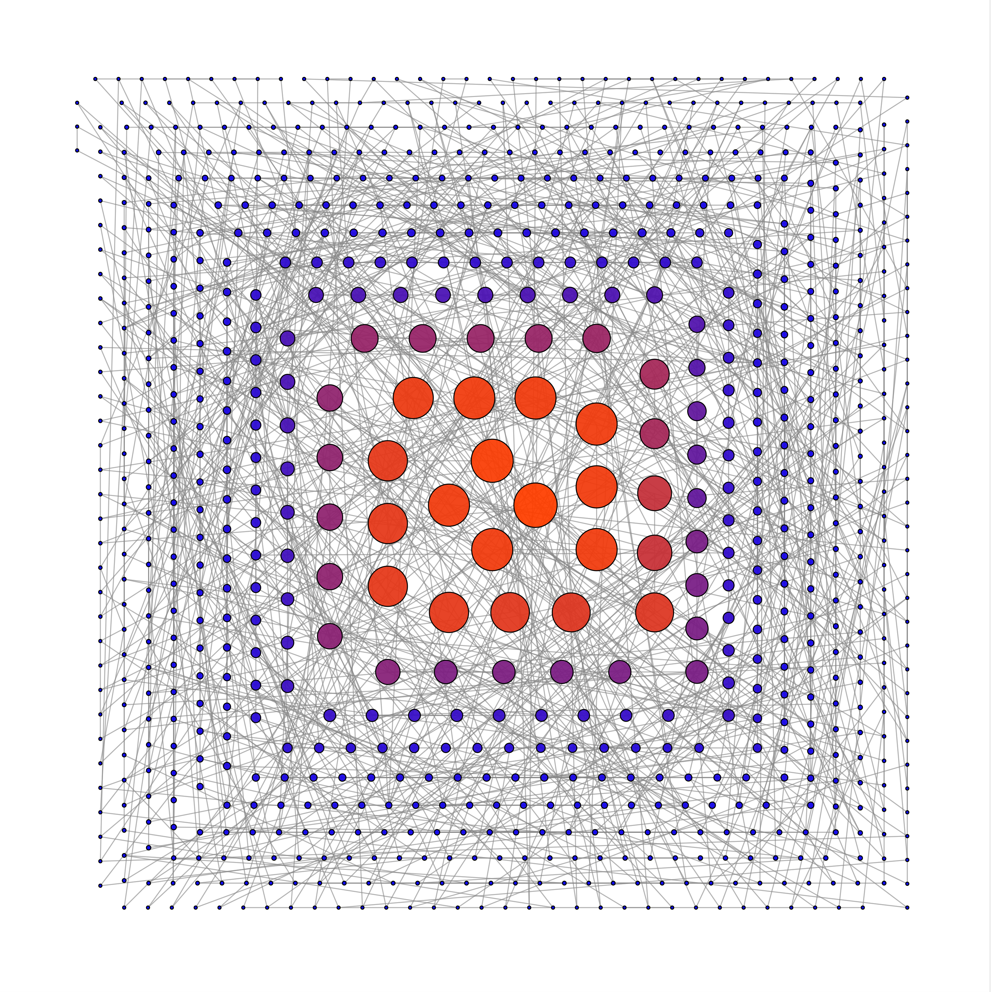
\includegraphics[scale=0.6]{tools/minecraft_4.png}
	\caption{Спиральная матричная визуализация на основе центральности саундтрека игры Minecraft}
\end{figure}

\begin{figure}[h]
	\centering
	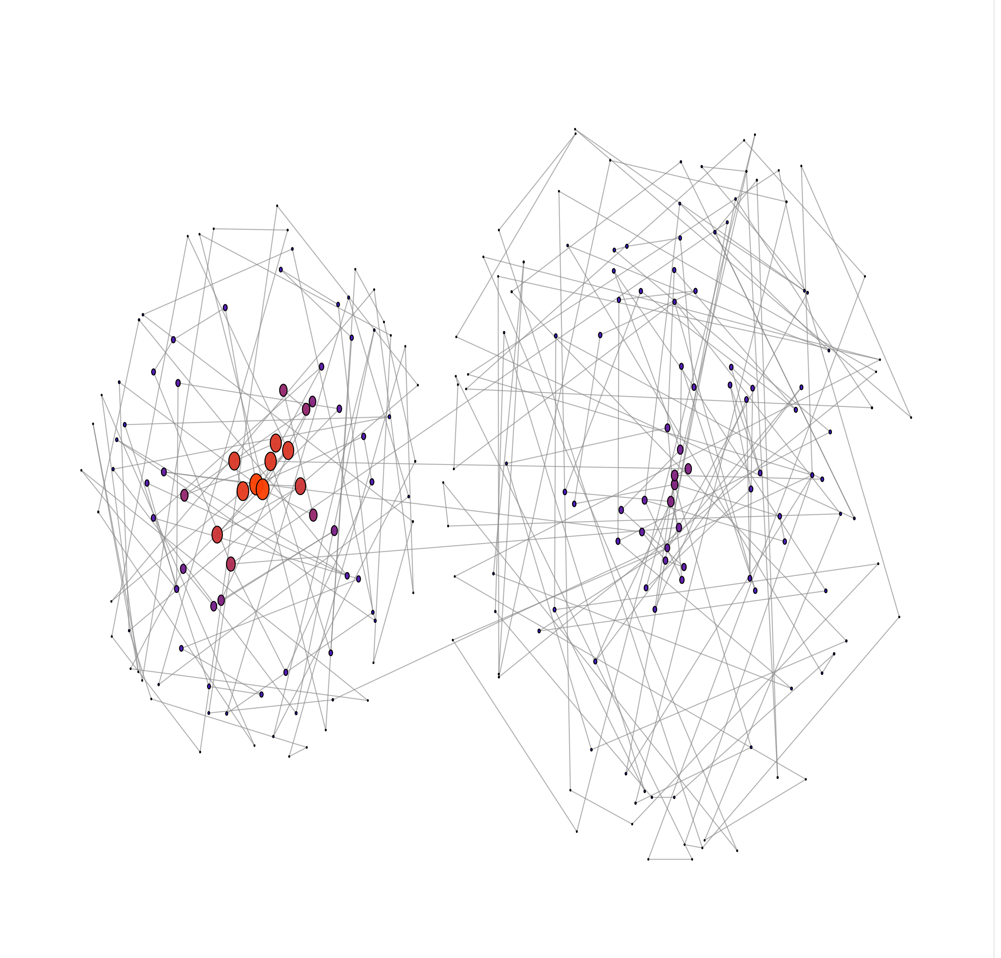
\includegraphics[scale=0.6]{tools/space_1.png}
	\caption{Визуализация трека Космос на основе модулярности Ньюмана}
\end{figure}

\begin{figure}[h]
	\centering
	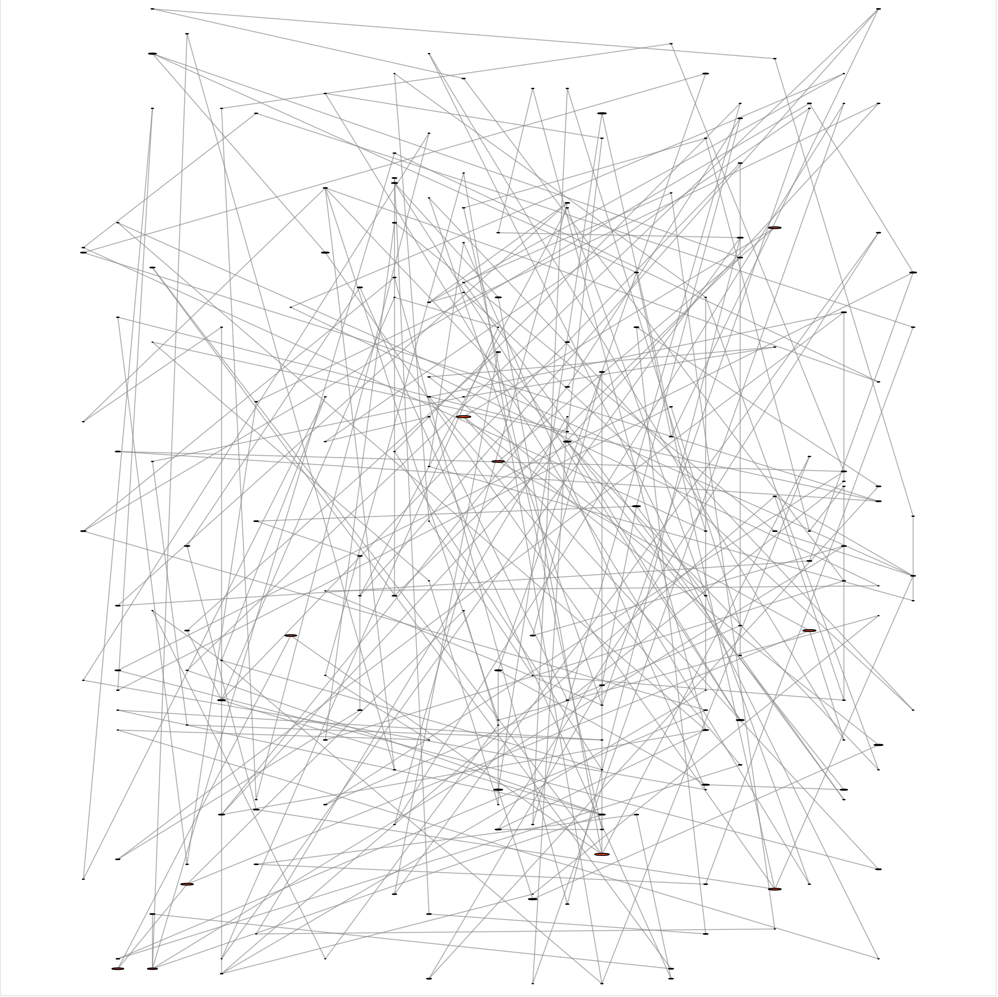
\includegraphics[scale=0.6]{tools/space_5.png}
	\caption{Визуализация графа-решетки трека Космос на основе центральности}
\end{figure}

\begin{figure}[h]
	\centering
	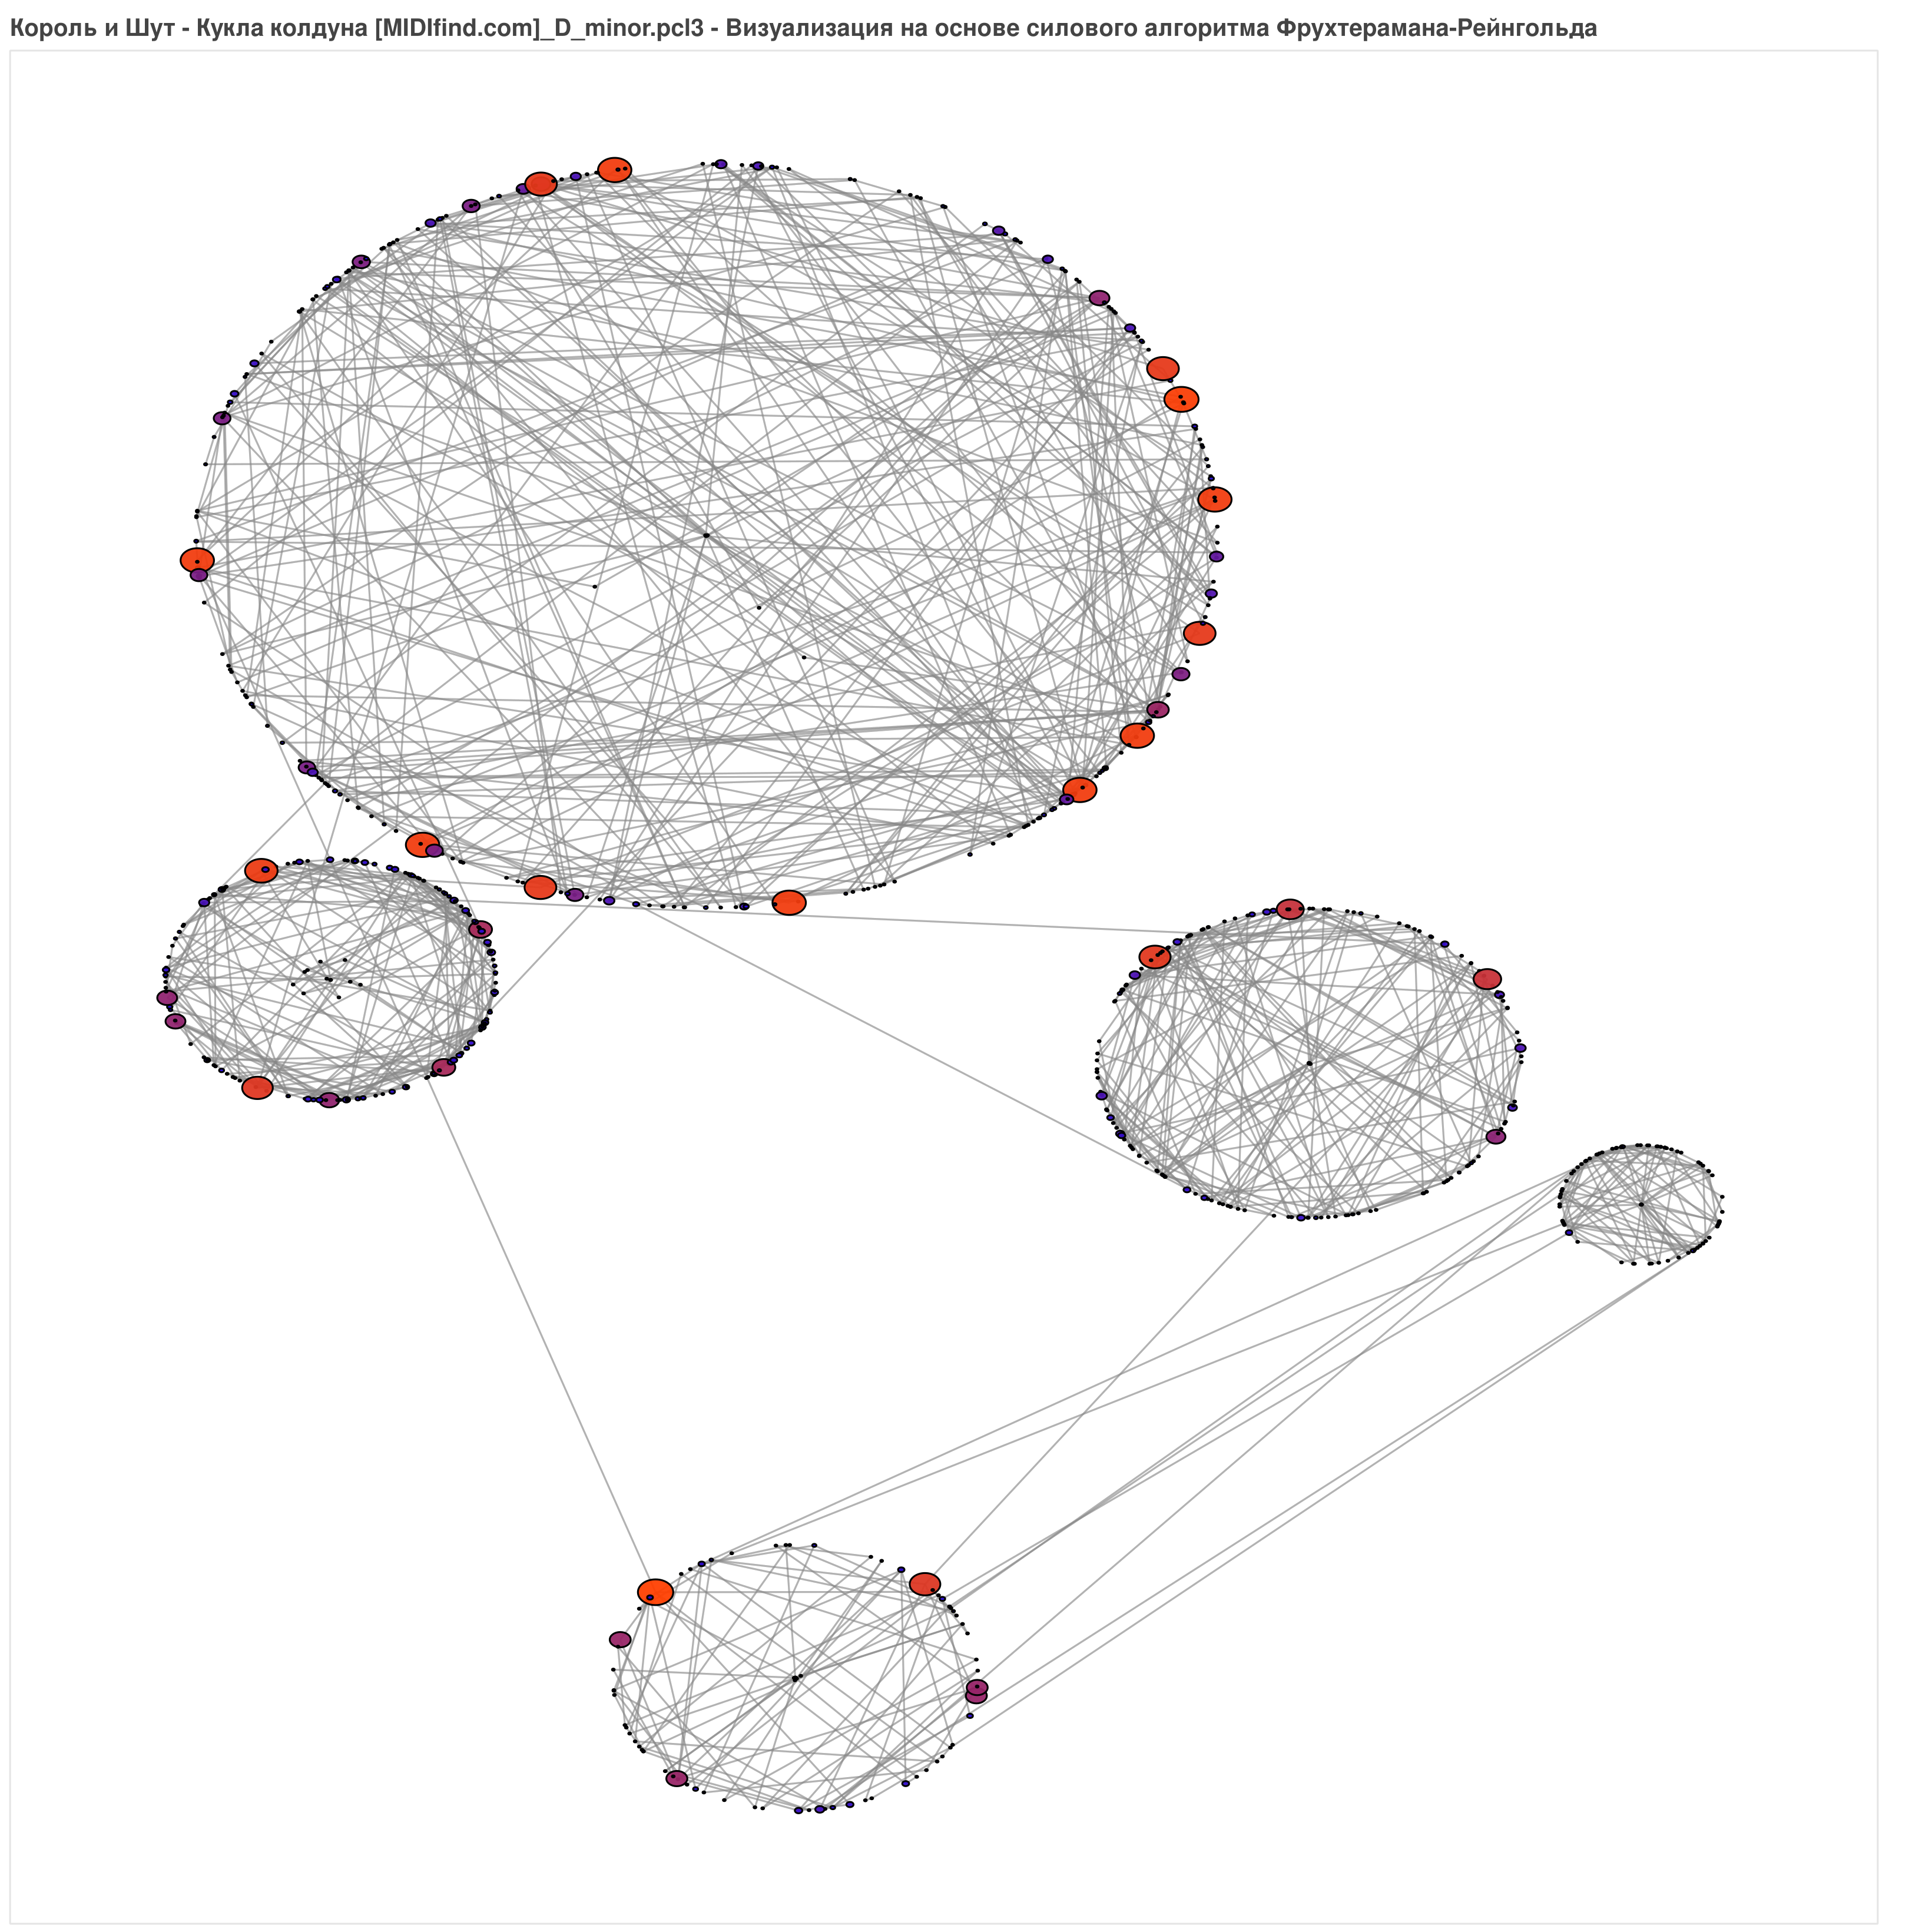
\includegraphics[scale=0.6]{tools/king_2.png}
	\caption{Визуализация трека Кукла колдуна на основе силового алгоритма Фрухтерамана-Рейнгольда}
\end{figure}

\begin{figure}[h]
	\centering
	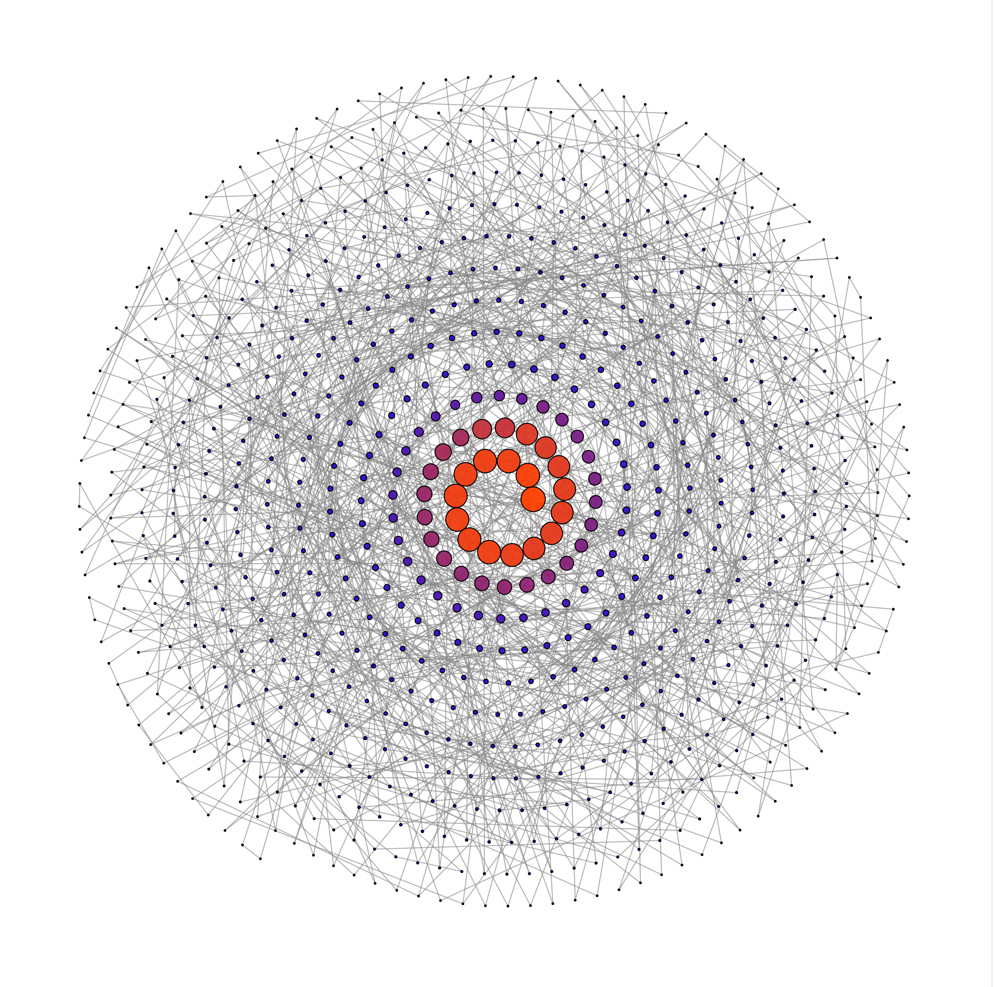
\includegraphics[scale=0.6]{tools/king_3.png}
	\caption{Спиральная визуализация на основе центральности трека Кукла колдуна}
\end{figure}

\begin{figure}[h]
	\centering
	\includegraphics[scale=0.6]{tools/groupblood_4.png}
	\caption{Спиральная матричная визуализация на основе центральности трека Группа крови}
\end{figure}

\begin{figure}[h]
	\centering
	\includegraphics[scale=0.6]{tools/groupblood_5.png}
	\caption{Визуализация графа-решетки трека Группа крови на основе центральности}
\end{figure}

\begin{figure}[h]
	\centering
	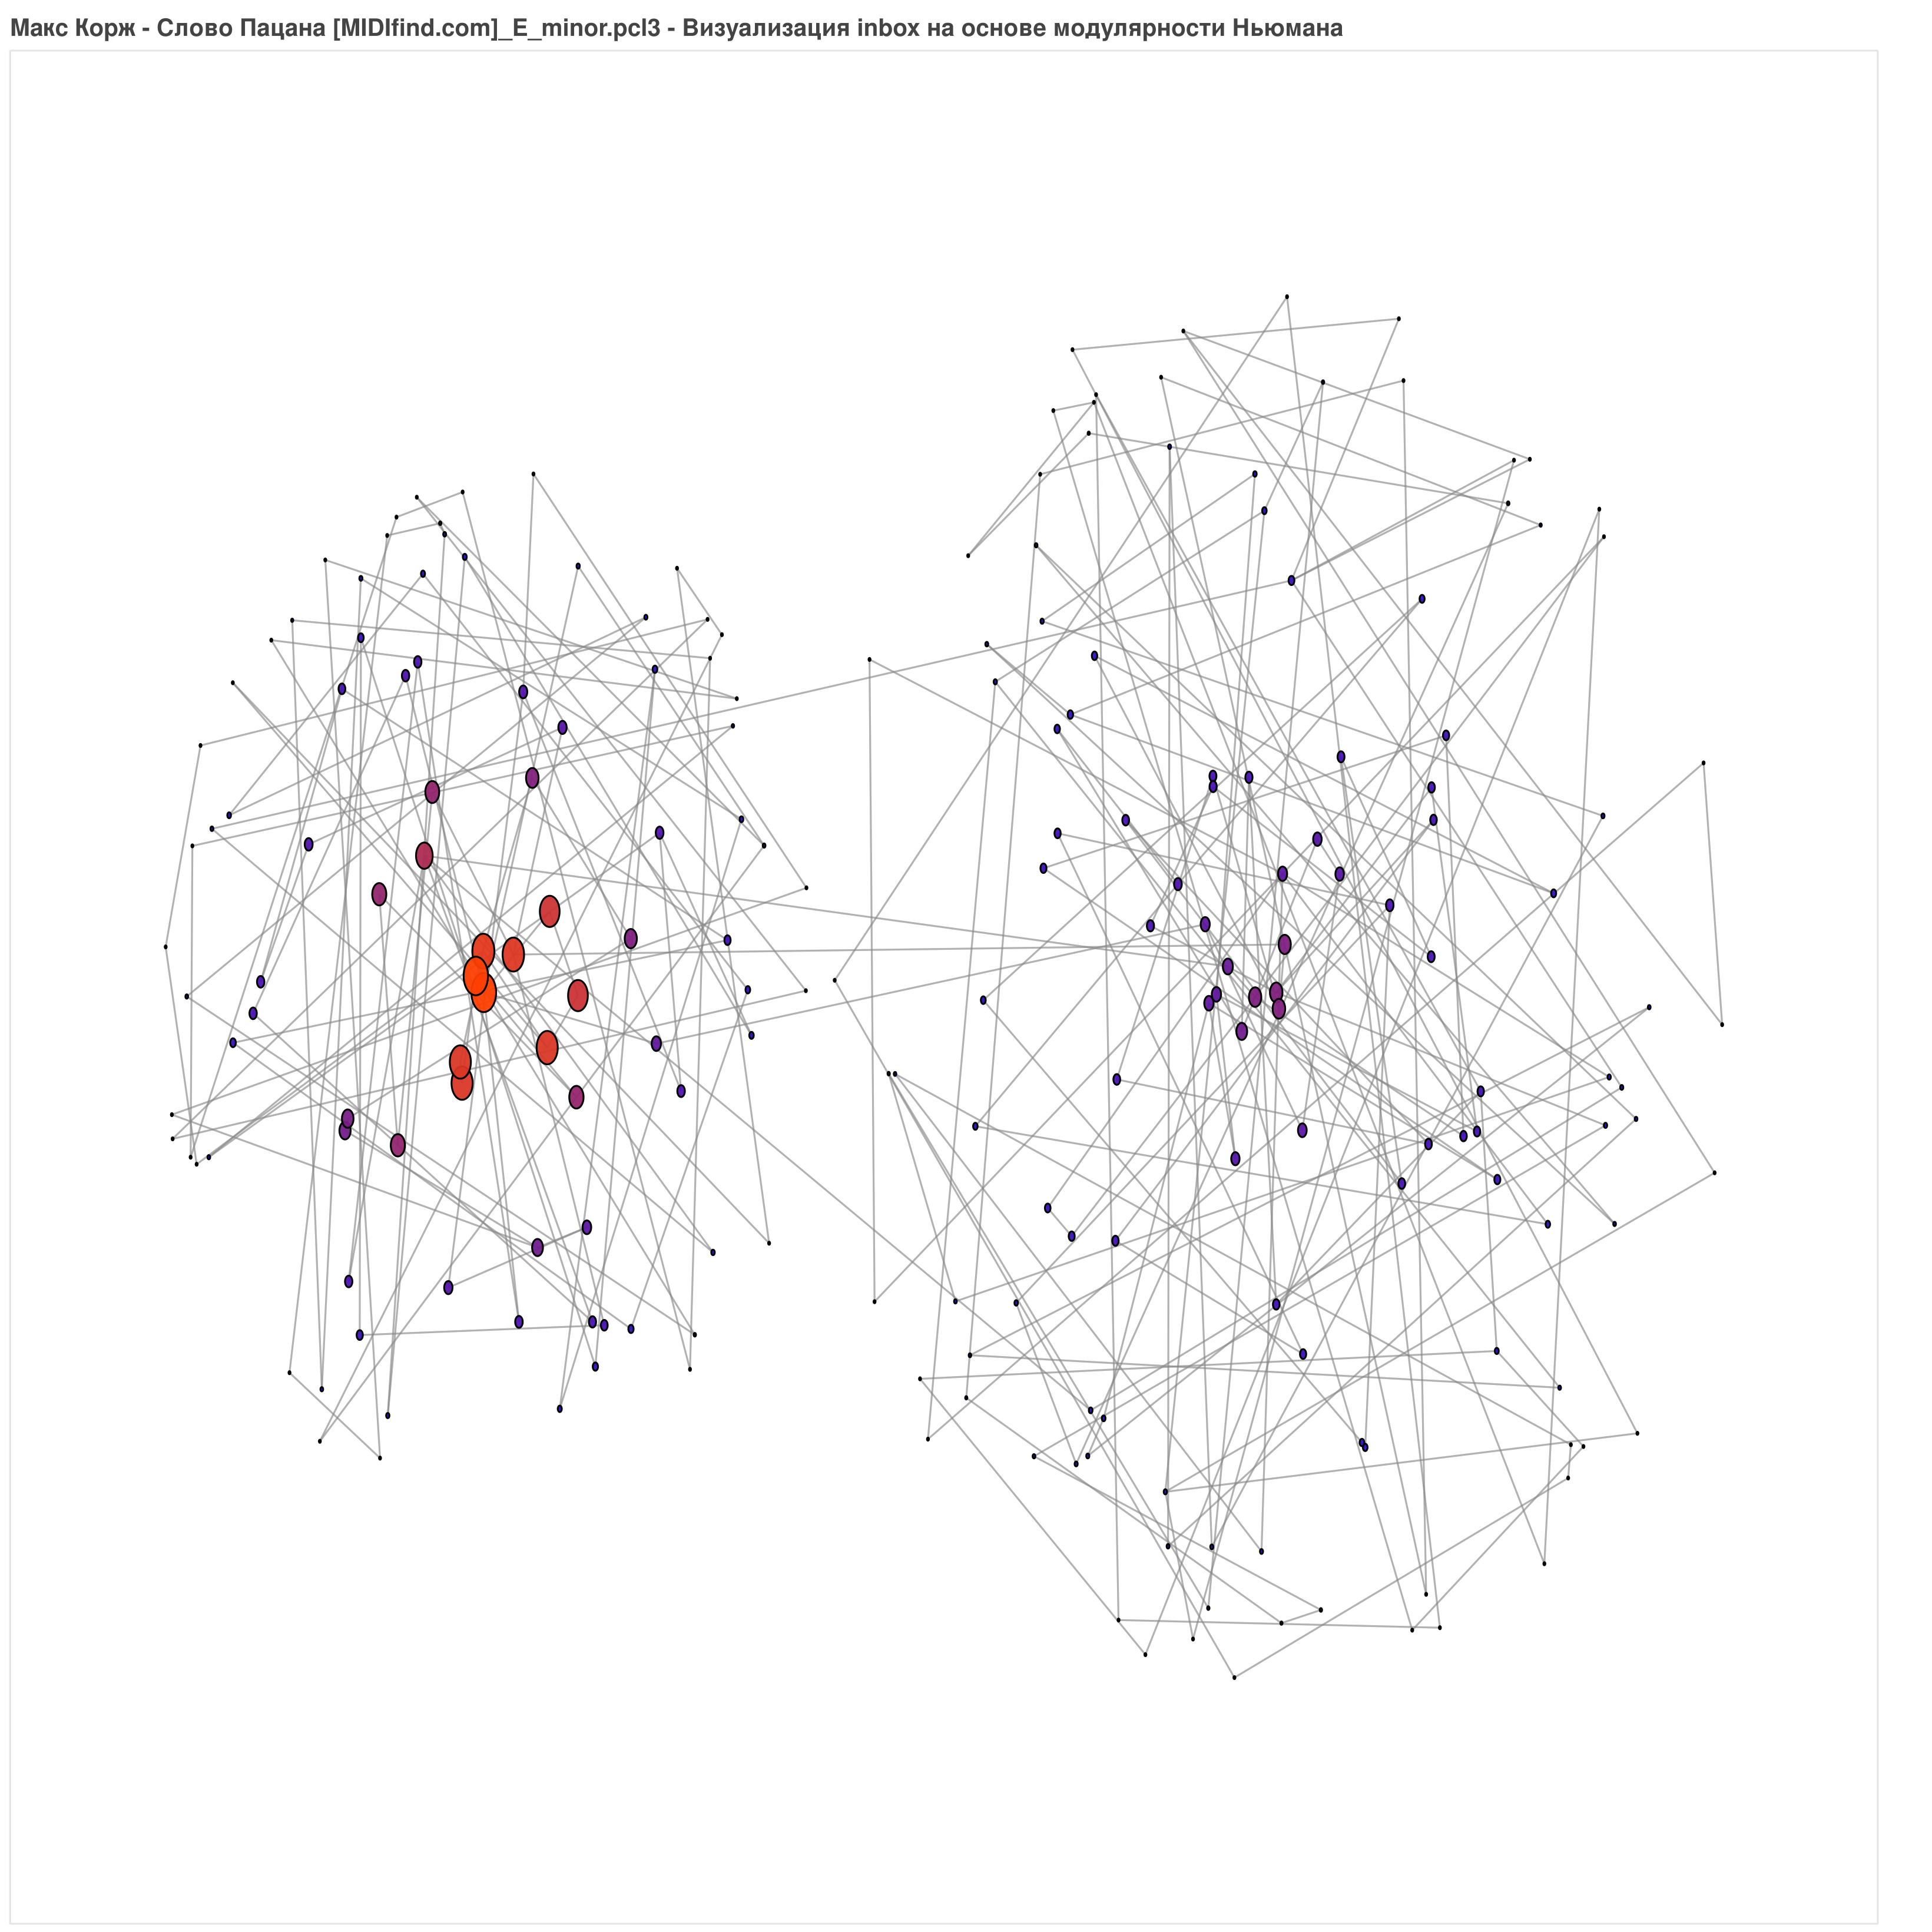
\includegraphics[scale=0.6]{tools/korj_1.png}
	\caption{Визуализация трека Слово пацана на основе модулярности Ньюмана}
\end{figure}

\begin{figure}[h]
	\centering
	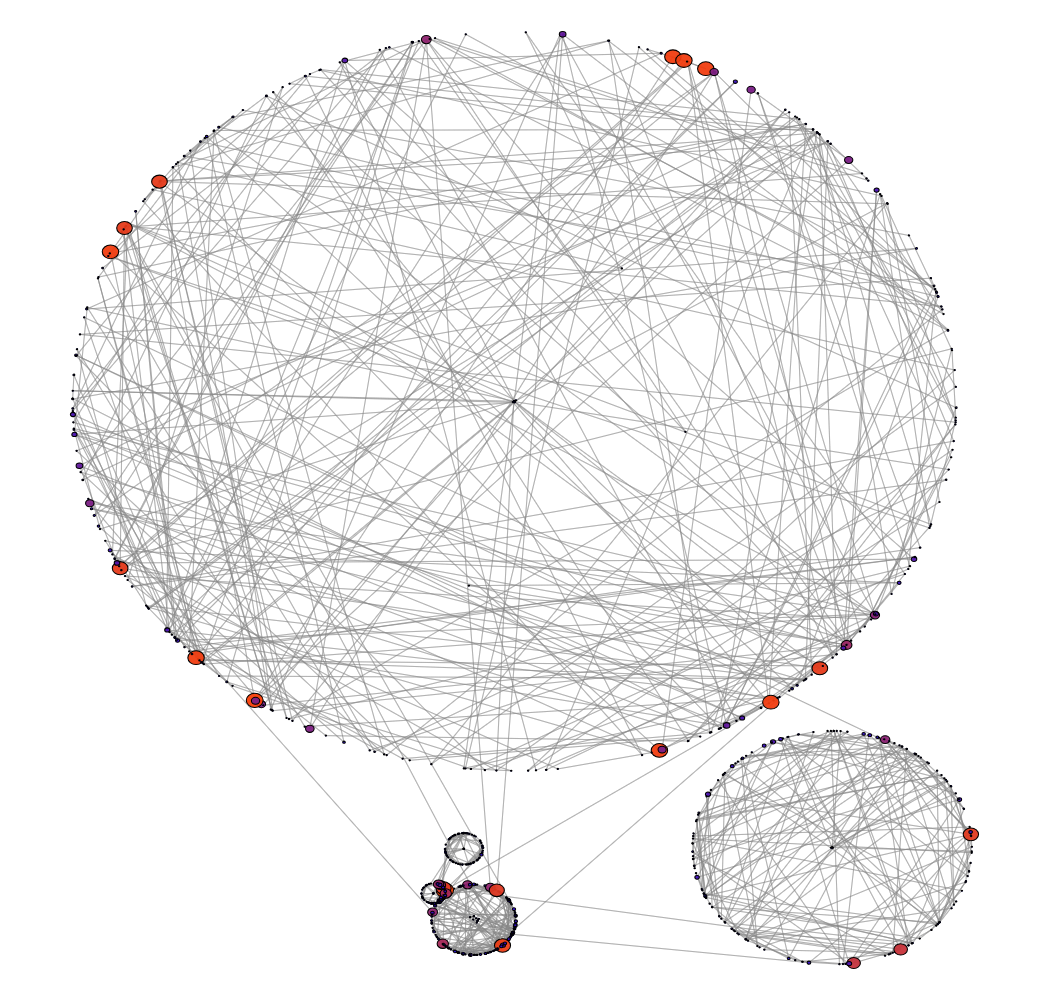
\includegraphics[scale=0.6]{tools/korj_2.png}
	\caption{Визуализация трека Слово пацана на основе силового алгоритма Фрухтерамана-Рейнгольда}
\end{figure}

\clearpage\section{Вывод}

В ходе работы были изучены принципы представления графов и их обработки с помощью вычислительного комплекса 
Тераграф. Получены графы для пяти треков. Графы строились пятью различными способами.

\end{document}